\chapter{Data-Engineering}
\label{ch:data}

\newcommand{\noaction}{37521\ }
\newcommand{\novideos}{194\ }
\newcommand{\nomatches}{152\ }

In diesem Kapitel werden die Schritte zur Generierung des Datensets SOCC-HAR-32 beschrieben, sowie seine Eigenschaften und weitere Aufbereitungsschritte.
Unter Data Engineering wird das Problem beschrieben, rohe Daten in ein \gls{ml}-Datenset zu transformieren~\cite{Burkov19}.
Dieser Prozess wird im Folgenden in zwei Teilprobleme unterteilt:
\begin{description}
    \item[Datenerhebung] Prozess, indem ein Datenset erstellt wird.
        Dazu werden verschiedene Datenquellen aggregiert und in einer Datenbank einheitlich persistiert.
    \item[Datenaufbereitung] Prozess zur Laufzeit des Trainings.
        Basierend auf dem Datenset, werden die persistierten Daten ausgelesen und dem \gls{har}-Modell in einer effizienten Weise bereitgestellt.
\end{description}

\begin{tcolorbox}[title=WIP]
    \begin{itemize}
        \item Plots (boxplot für Re-sampling, bar-plots drehen, sodass beschriftung leichter lesbar ist)
        \item Aktionskatalog im Anhang
        \item \Dh die Ungleichgewichtungen der realen Welt (insbesondere die Überrepräsentation von Background-Samples) wird auch im Test-Set widergespiegelt.
    \end{itemize}
\end{tcolorbox}


\section{Datenerhebung}
\label{sec:datenerhebung}

Das zu erstellende Datenset basiert auf den drei Datenquellen \gls{sbod}, SoccerNet und YouTube.
\gls{sbod} gibt eine Liste potenzieller Spiele und damit verknüpfter Spielaktionen vor, für welche passendes Videomaterial aus den anderen zwei Quellen gefunden werden muss.

\subsection{Datenschema}
\label{subsec:schema}

\begin{figure}
    \centering
    \bigimage{fig/schema}{0.7\textwidth}
    \caption{Datenbankschema zur Erhebung des Datensets}
    \label{fig:classes}
\end{figure}

Zu diesem Zweck wird zunächst ein einheitliches Datenschema bestend aus Spielen, Videos und Aktionen wie in \autoref{fig:classes} definiert.
Das Format bezieht sich auf die Speicherung aller Datenquellen in einer dokumentenbasierten NoSQL-Datenbank.

In SoccerNet werden stets zwei Videos pro Spiel bereitgestellt, wobei ein Video jeweils eine der zwei Halbzeiten zeigt.
Da diese Aufteilung nicht immer durch YouTube gegeben ist, werden im Falle eines kompletten Videos über beide Halbzeiten dennoch zwei Datensätze erstellt.
Beide Datensätze weisen dann die gleiche \code{externalId} (die sich aus der Video-\gls{url} ergibt) auf, markieren mit unterschiedlicher \code{startTime} und \code{endTime} jedoch disjunkte Intervalle innerhalb des Videos.

Die gesuchten Aktionsintervalle ergeben sich aus den Feldern \code{second} und \code{duration} und beziehen sich auf die jeweilige Spielzeit, beginnend mit dem Anpfiff der jeweiligen Halbzeit.
Die Zuordnung von Aktionen zu einem Teil-Datenset (\code{split}, hier: Trainings-, Validierungs-, Testset) geschieht Spiel-übergreifend.
\Dh alle Aktionen innerhalb eines Spiels werden stets dem gleichen Datenset zugeordnet.
Diese gängige Praxis wurde übernommen aus~\cite{Giancola18} und~\cite{Jiang19}.

\subsection{Verarbeitungs-Pipeline}
\label{subsec:pipeline}

Um die verschiedenen Datenquellen in das beschriebene Format zu überführen, wird ein semi-automatisierter Datenimport ausgeführt, deren Schritte in \autoref{fig:collection-pipeline_a} dargestellt sind.
Dieser überführt zunächst alle Spiele aus \gls{sbod} in das obige Datenschema.
Anschließend werden zwei Provider-Klassen (für SoccerNet und YouTube) implementiert, pro Spiel mehrere Stufen einer Import-Pipeline durchlaufen (\autoref{fig:collection-pipeline_b}), in denen weitere Datensätze angelegt werden.
Zuletzt werden die relationalen Daten aus der Datenbank in eine JSON-Datei exportiert.

\begin{figure}
    \centering
    \begin{subfigure}[b]{.5\textwidth}
        \centering
        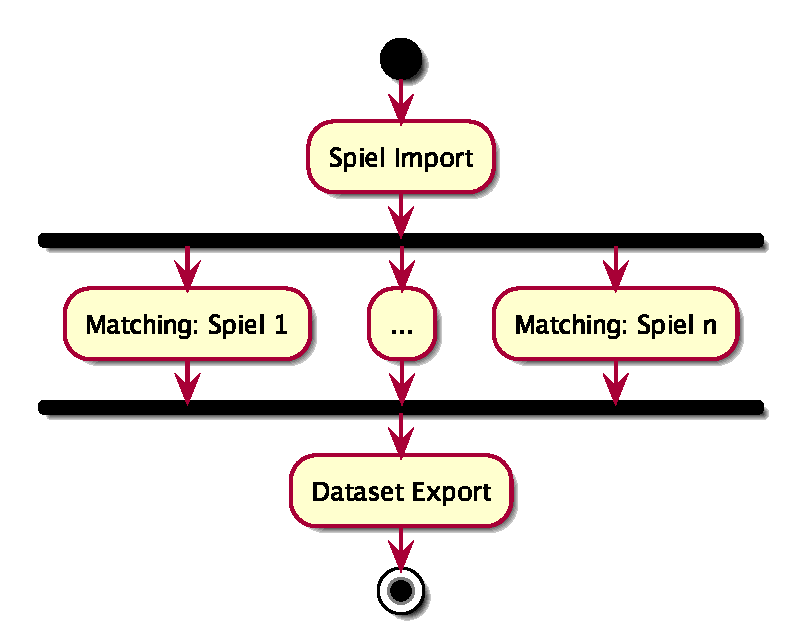
\includegraphics[width=.8\linewidth]{fig/collection.eps}
        \caption{Gesamter Prozess}
        \label{fig:collection-pipeline_a}
    \end{subfigure}%
    \begin{subfigure}[b]{.5\textwidth}
        \centering
        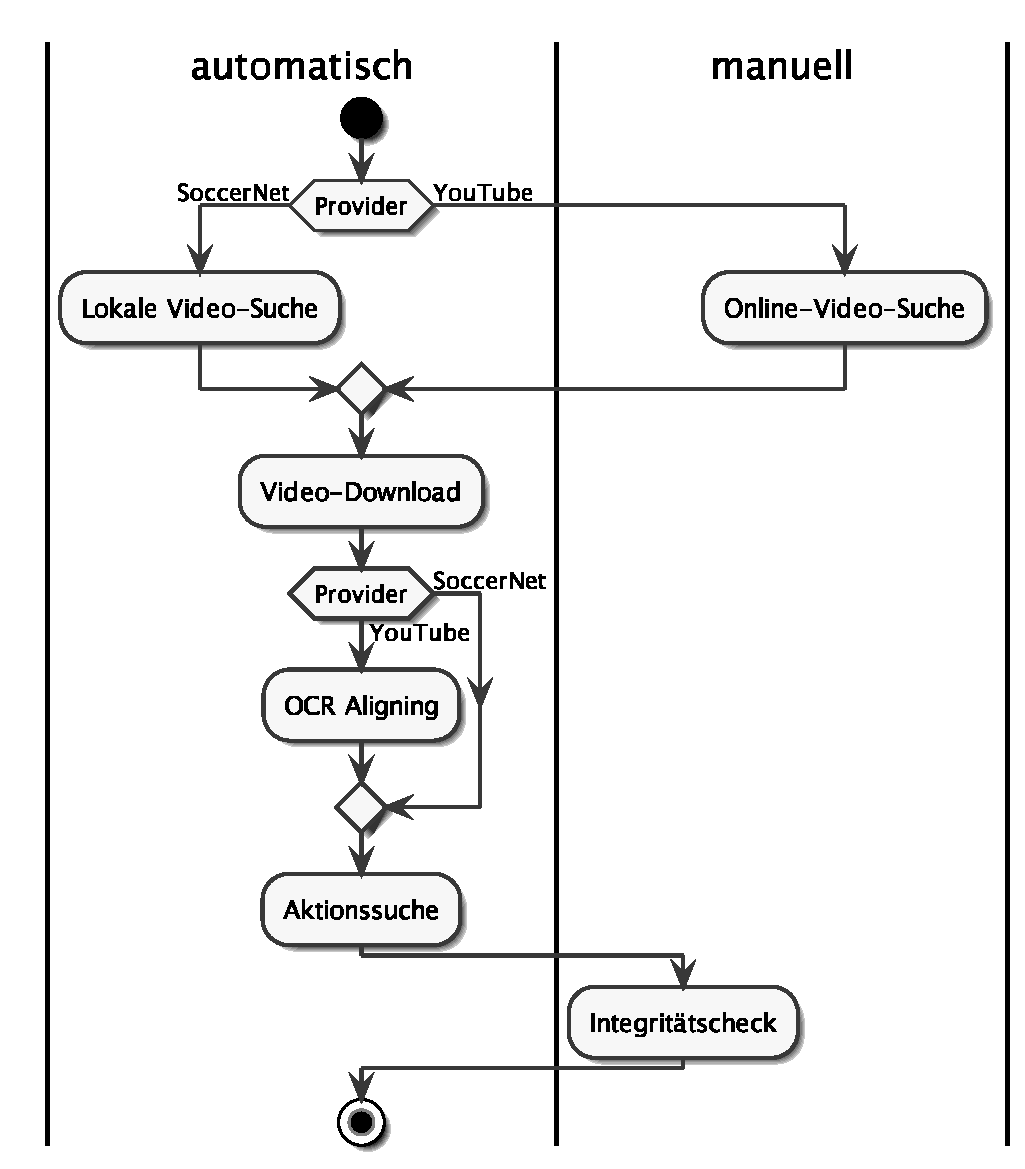
\includegraphics[width=.95\linewidth]{fig/collection-pipeline.eps}
        \caption{Matching pro Spiel}
        \label{fig:collection-pipeline_b}
    \end{subfigure}
    \caption{Pipeline zur Datenerhebung}
    \label{fig:collection-pipeline}
\end{figure}

Im ersten Schritt der Import-Pipeline wird ein Matching durchgeführt, welches prüft, ob es eine Überschneidung der Daten gibt.
Für den SoccerNet-Provider reicht ein lokaler Abgleich zwischen den online\footnote{https://github.com/SilvioGiancola/SoccerNet-code (Stand: 08.10.2020)} verfügbaren Dateilisten mit einem Suchbegriff -- bestehend aus Wettbewerb, Saison, Mannschaften, Spieldatum und Ergebnis.
Gibt es eine Übereinstimmung werden die Attribute \code{provider} und \code{externalId} des Matches gespeichert und jeweils zwei neue Video-Datensätze generiert.
Alle dieser Videos sind in je einer niedrigen (224p) und in einer hohen Qualität (720p oder 1080p) online verfügbar.
Zusätzlich wird pro Halbzeit eine Textdatei bereitgestellt, die den Zeitpunkt des An- und Abpfiffs innerhalb des Videos angibt.
Diese Informationen werden im jeweiligen Video-Datensatz als \code{startTime} bzw. \code{endTime} gespeichert.

Gibt es keine Übereinstimmung, wird auf den YouTube-Provider zurückgegriffen, der eine Online-Video-Suche anstößt.
Da Videos auf YouTube nicht für diese Aufgabe verifiziert sind, kann dieser Schritt nicht vollautomatisiert, sondern nur semi-automatisiert geschehen.
In einer \gls{gui} werden dem Nutzer mehrere Videos als Suchtreffer der YouTube-\gls{api} vorgeschlagenen.
Diese Videos kann der Nutzer mit den Eigenschaften des Match-Datensatzes (Datum, Ergebnis, Saison, etc.) manuell abgleichen und im Falle eines Matchings einer der Halbzeiten oder (falls das komplette Spiel gezeigt wird) beiden Halbzeiten zuordnen.
Wird bei keinem der Provider ein Treffer gefunden, wird das Spiel wieder aus der Datenbank gelöscht.

Im nächsten Schritt werden die Video-Dateien beider Halbzeiten in der höchstmöglichen Auflösung von der jeweiligen Plattform heruntergeladen und lokal zwischengespeichert.
Für alle Videos, die nicht vom SoccerNet-Provider kommen und somit noch keine \code{startTime} und \code{endTime} haben, wird die Startzeit der Halbzeit automatisiert mittels \gls{ocr} wie folgt bestimmt:

\subsubsection{Aligning mit OCR}

Damit die verfügbaren \gls{annotationen} mit den Video-Daten in Beziehung gesetzt werden können, müssen beide Datenquellen den gleichen zeitlichen Nullpunkt aufweisen.
Dieses Problem wird als Aligning bezeichnet~\cite{Purushwalkam20}.
Die \gls{sbod}-\gls{annotationen} bestimmen für jede Aktion einem Zeitpunkt gemessen an der Spieluhr (Spielzeit).
Die Videos selbst starten allerdings in der Regel schon wenige Minuten vor dem Anpfiff (Videozeit).
Als gemeinsame Nullpunkt wird deshalb der Anpfiff der jeweiligen Halbzeit festgesetzt.

In jedem Video befindet sich oben rechts oder oben links eine Spielzeitanzeige.
Der Nullpunkt im Video ist genau eine Sekunde bevor die Anzeige von \emph{00:00} aus \emph{00:01} umschlägt.

Um diesen Zeitpunkt schnell und genau zu finden, werden Screenshots verschiedener Frames erstellt, aus welchen mittels \gls{ocr} der Text des Bildbereichs extrahiert, indem typischerweise die Spieluhr zu finden ist.
Dieser Text, der immer dem Schema einer Uhrzeit entspricht, wird mit einem Regulären Ausdruck in Sekunden-Einheiten konvertiert, aus denen sich wiederum die Differenz von Videozeit zur Spielzeit ergibt.
Wiederholt man diesen Prozess oft genug, nähert sich der Median dieser Differenzen dem gesuchten Nullpunkt für den Anpfiff der ersten \bzw zweiten Halbzeit an.
Der Nullpunkt wird als \code{startTime} gespeichert, während sich die \code{endTime} aus Startzeit und Dauer der Halbzeit ergibt, wobei die Halbzeitdauer wiederum in den \gls{sbod}-\gls{annotationen} enthalten ist.
Der Einsatz einer \gls{ocr} wurde in ähnlicher Form auch in~\cite{Giancola18} für den gleichen Zweck genutzt.
Für die Umsetzung bedient sich diese Arbeit an der Open-Source-Bibliothek Tesseract~\cite{Smith07}.

\subsubsection{Aktionssuche}

An dieser Stelle der Pipeline können \gls{annotationen} und Videos miteinander kombiniert werden.
Daher werden im nächsten Schritt alle Aktionen eines Spiels vom Datenprovider \gls{sbod} geladen.
Diese externen, aus den 33 Oberkategorien bestehenden Klassendefinitionen \cite{StatsbombDocs16} werden in neu abgeleitete Aktionsklassen transformiert.

In \autoref{lst:sbod} ist ein exemplarischer Auszug, der eine Annotation aus \gls{sbod} zeigt.
Die Aktionsdatensätze der Datenbank beinhalten neben der \code{externalClass} (hier: übernommen aus Zeile 10), auch die weiteren Aktionsdetails (hier: ab Zeile 26) als \code{details}, aus denen neue, eigene Aktionsklassen abgeleitet werden.
Die neuen Aktionen werden durch einen Query-Selektor im MongoDB-Format\cite{Bradshaw16} definiert.
Mit dem Selektor können alle \gls{annotationen} dieser Klasse in einem Zug aus den \gls{sbod}-\gls{annotationen} eines Spiels, die in separaten Dateien vorliegen, gefiltert werden.
Die Repräsentation als Selektor ist unabhängig vom hier benutzten Datenschema und der Programmiersprache und lässt sich auch direkt auf die \gls{json}-\gls{annotationen} in \gls{sbod} anwenden.

%\lstinputlisting[language=json, caption=Datenformat in SoccerNet]{code/soccernet.json}
%\label{src:soccernet}

\lstinputlisting[language=json, label=lst:sbod, caption=Datenformat in Statsbomb Open Data]{code/sod.json}

\subsubsection{Integritätscheck}

Abschließend wird manuell noch die Überlagerung von Aktionen und Videos manuell kontrolliert.
Dabei wird geprüft, ob das Aligning korrekt ist, indem der Nutzer pro Halbzeit die Videozeit der ersten und letzten Spielminute in einer \gls{gui} verifiziert.
Dazu wird das Video in die \gls{gui} geladen und es wird zu der jeweiligen Stelle im Video gesprungen, in der das Aligning die zweite \bzw letzte Spielminute vermutet.
Sieht der Nutzer nun \zB die Spieluhr mit der Anzeige \emph{01:00} bzw. \emph{44:00} (bei punktgenauem Abpfiff) kann er das Alignment verifizieren.
Dadurch wird sichergestellt, dass keine Spielminuten aus dem Video herausgeschnitten wurden und dass die Abspielgeschwindigkeit der Originalgeschwindigkeit entspricht.

Als zweiter Integritätscheck wird geprüft, ob der zeitliche Nullpunkt dem tatsächlichen Anstoß entspricht.
Während der Entwicklungsphase hat sich herausgestellt, dass die eingeblendete Spieluhr nur in 7 \% der Fälle mit dem Anstoß beginnt zu zählen.
In 2,3 \% der Fälle startet sie bereits früher und in 90,8 \% erst später.
Die \gls{annotationen} in \gls{sbod} beziehen sich auf den \emph{echten} Nullpunkt, welcher sich durch den Anstoß definiert, was die Ergebnisse des vorherigen Alignings diskreditiert.
Denn ein fehlerhaftes Alignment führt zu einer systematischen Verschiebung aller Aktionsintervalle entlang der Zeitachse.

Um den potenziell falsch ermittelten Nullpunkt des Alignings zu korrigieren, kann der Nutzer den Nullpunkt in der \gls{gui} um wenige Sekunden nach vorne oder nach hinter justieren.
Zur Orientierung werden die Aktionen dabei unter dem Video in einer Zeitleiste eingeblendet.

Ist der Integritätscheck durch den Nutzer abgeschlossen, wird das Spiel einem der drei Datensubsets (Trainings-, Validierungs- und Testset) zugewiesen.
Bei Überschneidungen mit SoccerNet wird die Original-Zuteilung übernommen.
In allen anderen Fällen geschieht die Zuweisung zufällig unter der Gewichtung $3:1:1$ -- wie in~\cite{Giancola18}.

\subsubsection{Export}

Der letzte Schritt der Datenerhebung ist der Export in ein kompaktes Dateiformat, welches die Schnittstelle für weitere Anwendungen darstellt.
Das Zielformat ist eine Art Erweiterung des Speicherformats in~\cite{Caba15} (basierend auf JSON).
\autoref{fig:storage-format} zeigt das Format und hebt die Änderungen in Vergleich zum Basisformat hervor.

\begin{figure}
    \centering
    \bigimage{fig/storage}{0.7\textwidth}
    \caption{Dateiformat zur Speicherung des Datensets}
    \label{fig:storage-format}
\end{figure}

Die Liste der Klassen wird durch die in \autoref{subsec:pipeline} genannten Selektoren erweitert.
Die eigentliche Datenbank speichert Einträge pro Halbzeit in einer Map, wobei sich der Schlüssel der externen Spiel-ID aus \gls{sbod} und der Nummer der Halbzeit zusammensetzt.
Pro Halbzeit kann über die \gls{url} auf das Video geschlossen werden.
Da sich das Video potenziell mit der anderen Halbzeit desselben Spiels überschneidet, wurden zusätzlich die Start- und Endzeit der Halbzeit unter \code{segment} gespeichert.
Jede Videohälfte referenziert nun eine Liste der darin enthaltenen Aktionen mit jeweils dem \code{label} und einem \code{segment} bestehend aus Start- und Endmarkierung.
Zusätzlich wird auch hier ein eindeutiger Identifier in Form einer \gls{url} definiert, um das Debugging zu erleichtern.

\section{Eigenschaften des Datensets}
\label{sec:eigenschaften-des-datensets}

Das Resultat der Datenerhebung ist ein Datenset, welches \noaction Aktionen und \novideos Videos aus insgesamt \nomatches Spielen umfasst.
In \autoref{tab:action} werden alle 32 Klassen des Datensets aufgelistet.
Neben der Anzahl ist die durchschnittliche und maximaler Dauer pro Aktion vermerkt, die sich aus den \gls{annotationen} in~\cite{Statsbomb20} ergeben.
Aktionen, die hier keinen Wert vorweisen werden lediglich als Zeitpunkt in \gls{sbod} repräsentiert.

\begin{figure}
    \centering
    \small
    \begin{subfigure}{0.45\textwidth}
        \centering
        \csvautotabular{tbl/actions_a.csv}
    \end{subfigure}
    \begin{subfigure}{0.45\textwidth}
        \centering
        \csvautotabular{tbl/actions_b.csv}
    \end{subfigure}
    \caption{Aktionskatalog in SOCC-HAR-32}
    \label{tab:action}
\end{figure}

\subsection{Ungleichverteilung von Aktionen}
\label{subsec:ungleichverteilung-von-aktionen}

Trotz der hohen Zahl an Aktionsklassen, besteht der Hauptteil des Videomaterials aus aktionsfreien Teilen (Background).
\autoref{fig:anno_bg_ratio} zeigt das Verhältnis von durch Aktionen geprägter Videozeit bei einsekündiger Segmentierung aller Halbzeitvideos.
Die Zeit vor und nach den Halbzeiten wird nicht mitgezählt.
Hinzu kommt, dass die Klassen untereinander sehr ungleich verteilt sind, wie \autoref{fig:anno_classes} zeigt.
Die genauen Zahlen sind ebenso der Tabelle in \autoref{tab:action} zu entnehmen.

\begin{figure}
    \centering
    \begin{subfigure}{.5\textwidth}
        \centering
        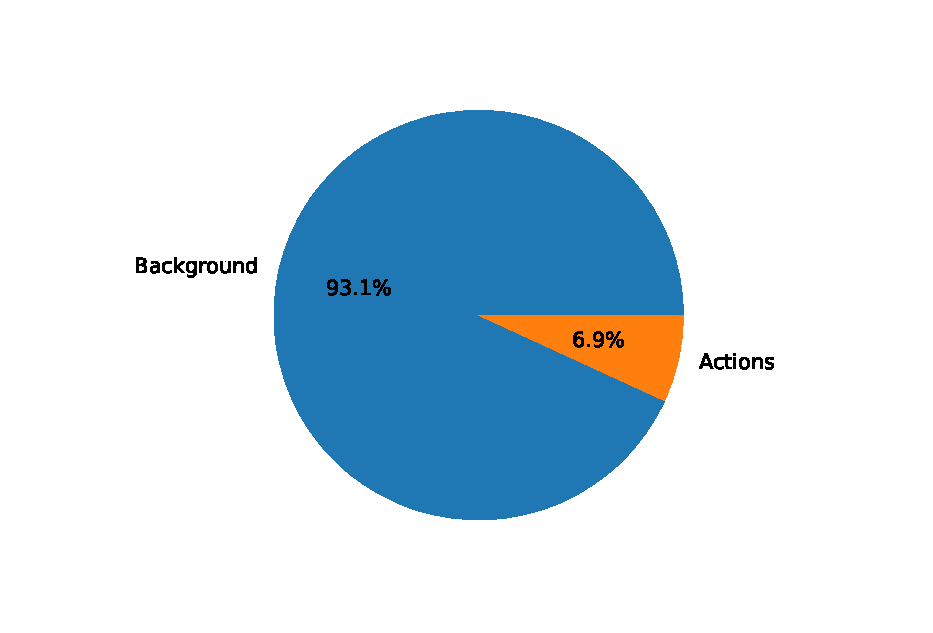
\includegraphics[width=.9\linewidth]{img/data-plots/background_ratio_all_annos.eps}
        \caption{Anteil der Aktionen im Videomaterial}
        \label{fig:anno_bg_ratio}
    \end{subfigure}%
    \begin{subfigure}{.5\textwidth}
        \centering
        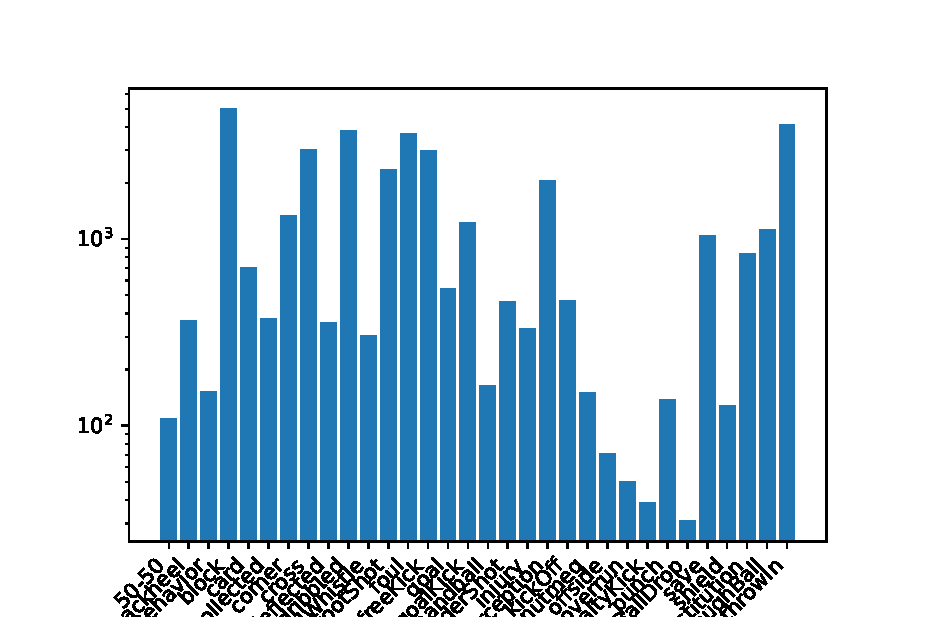
\includegraphics[width=.95\linewidth]{img/data-plots/class_distribution_annotations_all.eps}
        \caption{Verteilung der Klassen}
        \label{fig:anno_classes}
    \end{subfigure}
    \caption{Eigenschaften zum Datenset}
    \label{fig:annotations}
\end{figure}


\subsection{Überschneidungen von Aktionen}
\label{sec:multi-label}

Der oben genannte Aktionskatalog hat mit insgesamt 32 Aktionsklassen das Potenzial einige Aktionen zu beinhalten, die sich mit anderen zeitlich überschneiden.
Dazu zählt einerseits der Fall, dass zwei Aktionen von zwei verschiedenen Spielern tatsächlich zeitgleich ausgeführt werden.
Andererseits können abhängig von der Problembeschreibung \zB hierarchische Klassen definiert werden, sodass sich eine Klasse \code{penaltyKick} immer mit der Klasse \emph{footShot} überlagert.

Um die Signifikanz dieses Problems zu verdeutlichen wurden untersucht, wie sich die Wahl von $\Delta$ auf die Anzahl von Überschneidungen auswirkt.
\autoref{fig:ratios} zeigt, dass bei einem höheren Zeitkontext $\Delta$ die Zahl von Hintergrund-Samples zwar sinkt, die Zahl der Überschneidungen jedoch steigt.

Als Folge der oben veranschaulichten Statistiken wird vorab auf ein Multi-Label-Ansatz gesetzt.
Das Verfahren ist damit auch flexibler bei Anpassungen des Aktionskatalogs und kommt ohne ein künstlichen \emph{Background}-Labels aus.
Zudem kann auf ein aufwendiges Verfahren dedizierte, überschneidungsfreie Intervalle für jede Aktion zu finden, verzichtet werden.
Stattdessen kann das ungeschnittene Videomaterial gleichmäßig in Clips segmentiert werden und jeder Clip erhält ein Label pro darin stattfindender Aktion.

Zudem wurde untersucht, wie oft sich eine Klasse mit einer anderen überschneidet.
Eine dedizierte Grafik ist in \autoref{ch:overlaps} zu finden.
Die häufigsten Kombinationen sind (bei $\Delta=4$) folgende:

\begin{enumerate}
    \item \code{saved} mit \code{footShot}: 74 \%
    \item \code{penaltyKick} mit \code{goal}: 57 \%
    \item \code{badBehavior} mit \code{card}: 51 \%
    \item \code{goal} mit \code{footShot}: 50 \%
    \item \code{collected} mit \code{cross}: 40 \%
\end{enumerate}

\begin{figure}
    \centering
    \begin{subfigure}{.3\textwidth}
        \centering
        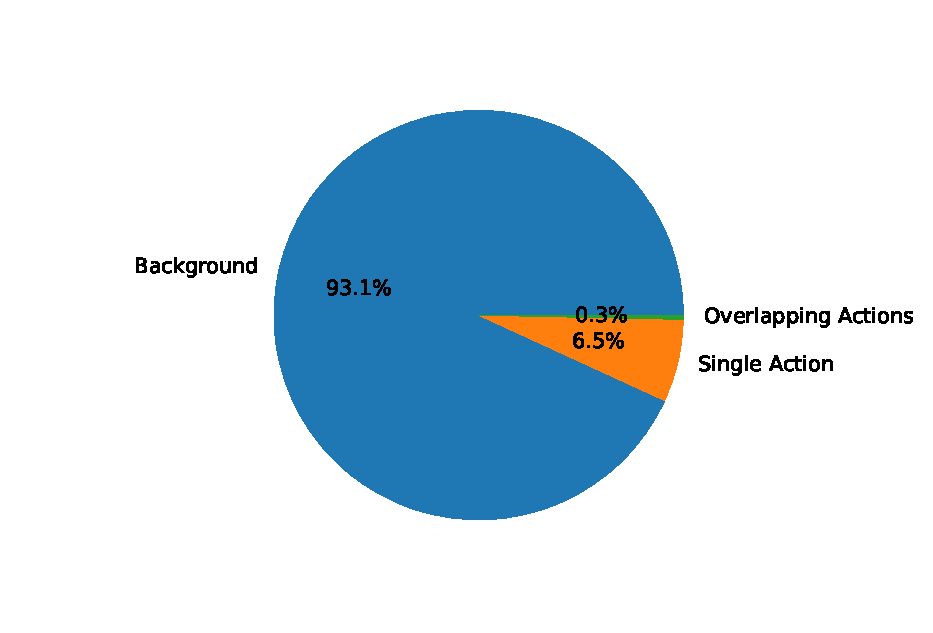
\includegraphics[width=.95\linewidth]{img/data-plots/1sec/background_ratio_all_1sek.eps}
        \caption{$\Delta = 1$}
        %\label{fig:anno_bg_ratio}
    \end{subfigure}%
    \begin{subfigure}{.3\textwidth}
        \centering
        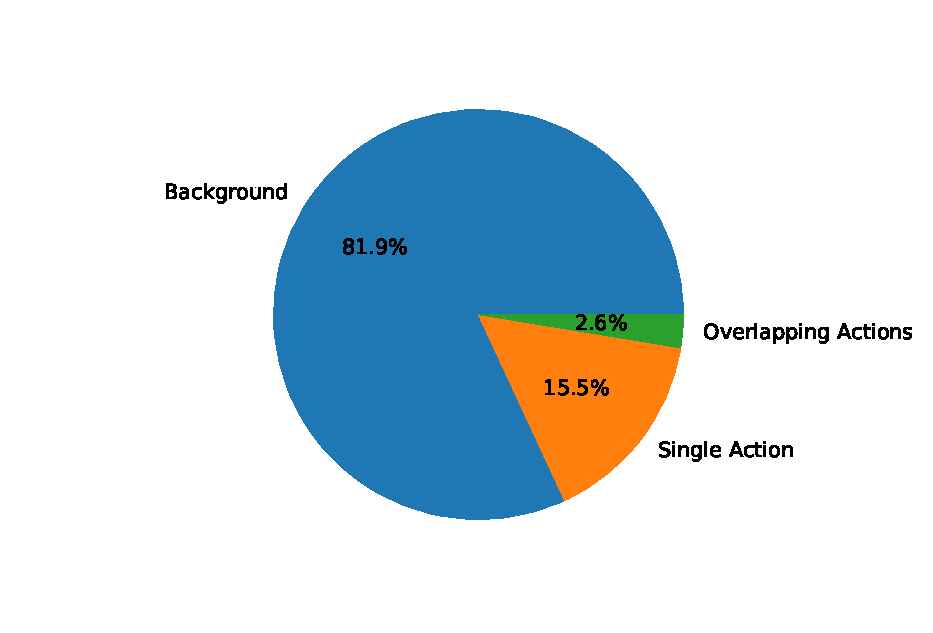
\includegraphics[width=.95\linewidth]{img/data-plots/4sec/background_ratio_all_202010-1419-3706.eps}
        \caption{$\Delta = 4$}
        %\label{fig:anno_classes}
    \end{subfigure}
    \begin{subfigure}{.3\textwidth}
        \centering
        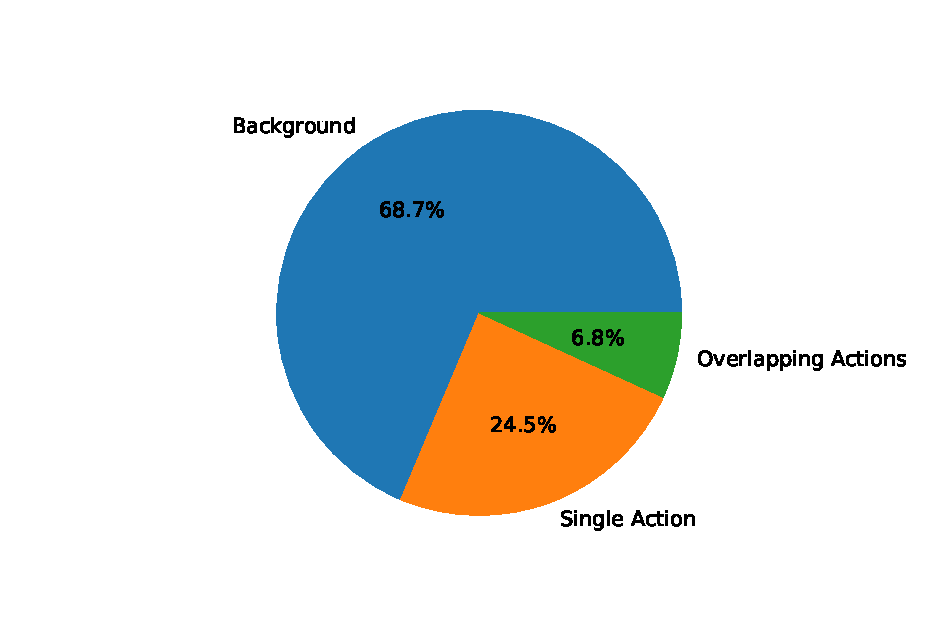
\includegraphics[width=.95\linewidth]{img/data-plots/8sec/background_ratio_all_202010-1419-4303.eps}
        \caption{$\Delta = 8$}
        %\label{fig:anno_classes}
    \end{subfigure}
    \caption{Skalierung des Background- und Überschneidungsverhältnisses zur Wahl von $\Delta$}
    \label{fig:ratios}
\end{figure}

\section{Datenaufbereitung}
\label{sec:pre-processing}

Die Datenaufbereitung basiert auf dem exportierten Datenset des vorherigen Kapitels.
Es umschließt einmalige Prozesse, sowie Prozesse, die pro Training oder pro Sample während des Trainings durchgeführt werden.
\autoref{fig:data-pipeline} zeigt die Prozesse jeder dieser Kategorien.

\begin{figure}
    \centering
    \bigimage{fig/data-pipeline}{0.7\textwidth}
    \caption{Pipeline zum Pre-Processing basierend auf Annotationen}
    \label{fig:data-pipeline}
\end{figure}

\subsection{Effizientes Laden und Speichern}
\label{subsec:effiziente-speicherung}

Um Samples $(x_i, y_i)$ aus den Videos des Datensets zu generieren, müssen einzelne Frames aus den Videos extrahiert und in den Arbeitsspeicher geladen werden.
Dieser Prozess wiederholt sich für jedes Sample pro Epoche, die trainiert wird und stellt ohne weitere Optimierungen einen enormen IO-Overhead dar, der die Geschwindigkeit des eigentlichen Trainings ausbremsen kann~\cite{Wu20}.
Der IO-Zugriff kann \zB reduziert werden, indem die relevanten Frames vorab extrahiert und als Bilder gespeichert werden.
Dieses Vorgehen skaliert jedoch nur mäßig mit der Größe des Datensets, da die Bilder schon bei kleinen Datensets oft zu viel Speicherplatz einnehmen.
Alternativ kann der Zugriff durch Multiprocessing optimiert werden und indem die Videos vorher analysiert werden.
Sind Framerate und \gls{pts} eines Videos bekannt, kann mithilfe des \gls{pes} die entsprechende Stelle innerhalb des Videos direkt und vergleichsweise schnell gefunden werden~\cite{Fischer10}.
Diese Methode ist in den einschlägigen \gls{har}-Bibliotheken (darunter auch die Implementationen von~\cite{Feichtenhofer18} und~\cite{Wang19}) gängige Praxis und wird in diesem Setup übernommen.

Da die Videos nun on-demand dekodiert werden müssen, werden die Videos schon im Vorhinein in einer geringen Auflösung heruntergeladen werden.
Als Zielauflösung wird 360p festgelegt, da es immer noch ein Cropping des höchstauflösenden Modells (mit $S=312$) zulässt und gleichzeitig eine gängige Auflösung des Providers YouTube ist.

Die Videos des Providers YouTube können direkt in der Zielauflösung heruntergeladen werden.
Die Videos des Providers SoccerNet müssen hingegen erst in High Definition heruntergeladen werden und anschließend in die Zielauflösung konvertiert werden.
Alle Videos haben eine einheitliche Framerate von 25 \gls{fps}.
Sobald ein Video in der Zielauflösung verfügbar ist, kann es analysiert werden.
Dazu werden die \gls{pts} und weitere Metadaten erhoben und in einer Pickle-Datei \cite{Lubanovic19} persistiert.

\subsection{Segmentierung und Sampling-Strategie}
\label{subsec:segmentierung-und-sampling-strategie}

Sind Videos und Metadaten lokal verfügbar, können die ungeschnittenen Videos zu \glspl{clip} segmentiert und gelabelt werden.
Die \glspl{clip} werden in einer konfigurierbaren Länge $T$ und Framerate gesamplet.
Um mehrere Samples aus den zugrundeliegenden \gls{annotationen} zu generieren, werden die \glspl{clip} mit einer Verschiebung von einer Sekunde gesamplet.
Das hat zur Folge, dass sich die \glspl{clip} (bei $T > \text{Framerate}$) überschneiden (Temporale Augmentation, siehe~\cite{Giancola18}) und so zusätzliche Samples aus der begrenzten Zahl an Annotationen entstehen.
\autoref{fig:samples} vergleicht pro Klasse die Anzahl möglicher Samples zur Anzahl bestehender \gls{annotationen} bei einer Dauer von $\Delta=4$ Sekunden.

\begin{figure}
    \centering
    \begin{subfigure}{.5\textwidth}
        \centering
        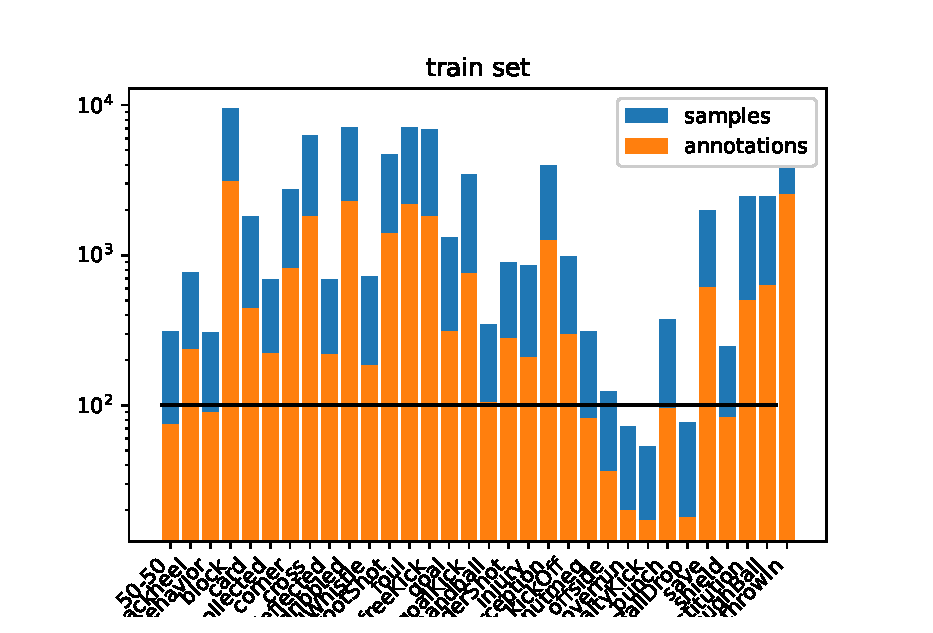
\includegraphics[width=.95\linewidth]{img/data-plots/4sec/class_distribution_annotations_train_202010-1419-3737.eps}
        \caption{Trainingsdaten}
        %\label{fig:anno_bg_ratio}
    \end{subfigure}%
    \begin{subfigure}{.5\textwidth}
        \centering
        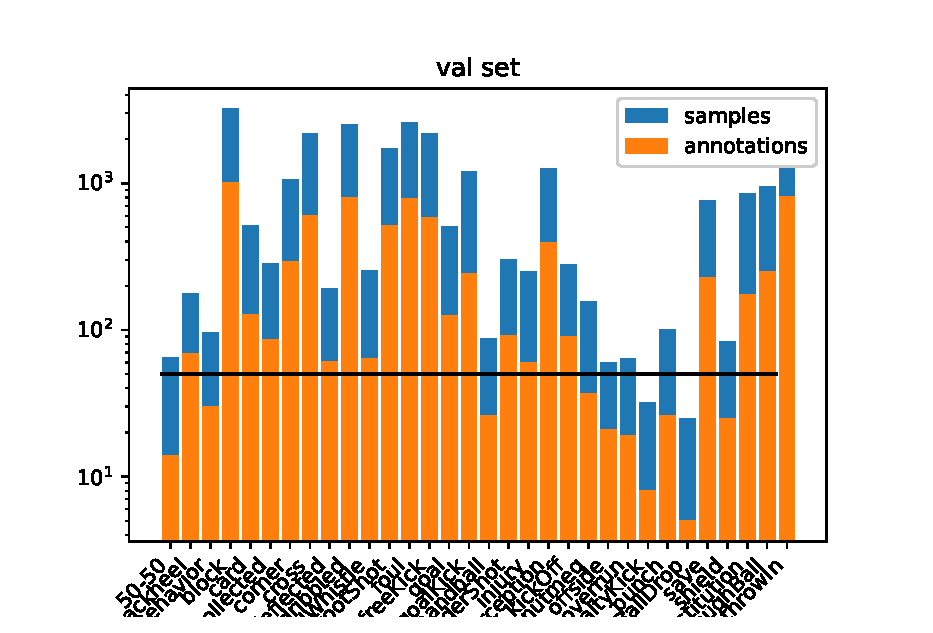
\includegraphics[width=.95\linewidth]{img/data-plots/4sec/class_distribution_annotations_val_202010-1419-3747.eps}
        \caption{Validierungsdaten}
        %\label{fig:anno_classes}
    \end{subfigure}
    \caption{Generierung zusätzlicher Samples aus den Annotationen (bei $\gls{tld:Delta} = 4.0$)}
    \label{fig:samples}
\end{figure}

Diese potenziellen Samples werden intern als Tripel aus Videopfad, Framerate und \gls{pts} gespeichert.
Da die Trainingslaufzeit proportional mit der Anzahl der Samples skaliert, muss die Gesamtzahl der Samples im Kontext dieser Arbeit jedoch deutlich reduziert werden.
Zum einen werden Samples, die keine Überschneidung mit einer der zwei Halbzeiten haben, aussortiert.
Ebenso werden kritische Samples entfernt, die keine Überschneidung mit einer Annotation haben (Background-Samples), aber einen sehr \emph{nahen} zeitlichen Abstand zur nächsten Aktion haben.
Motiviert ist diese Entscheidung durch die teils inakkuraten Segmentmarkierungen in den \gls{sbod}-\gls{annotationen}.
Die Grenzen einer Aktion sind teils subjektiv gelabelt und durch das Erlauben kritischer Background-Samples würde ein falsches Bild von Genauigkeit entstehen.
Als Folge wird erwartet, dass das Modell die Aktionsgrenzen implizit selbst erlernt und da Background-Samples ohnehin überrepräsentiert sind, wird nicht erwartet, dass es so zu Performance-Einbußen kommt.
Ein Background-Sample wird als kritisch deklariert, wenn es eine dreisekündige Pufferzone einer anderen Aktion schneidet, was laut \autoref{subsec:hyperparameter} etwa der durchschnittlichen Länge einer Aktion entspricht.

Zusätzlich wird die Maximalzahl an Samples pro Klasse durch einen Richtwert $\gls{tld:Theta}$ gedrosselt.
Der Richtwert für Trainingsdaten orientiert sich an~\cite{Kay17} (250-1000 Samples pro Klasse) und ist konfigurierbar.
Analog wird die Größe der Validierungs- und Testsamples fest auf 50 \bzw 100 Samples begrenzt.

Da es sich um ein Multi-Label-Datenset handelt, sind die Grenzwerte tatsächlich nur als Richtwerte anzusehen.
Denn bei einer harten Obergrenze würde in Kauf genommen werden, dass Samples einer unterrepräsentierten Klasse ebenfalls ausgeschlossen werden können, wenn sie in Kombination mit einer überrepräsentierten Klasse auftreten.

Die Auswahl der Samples pro Datenset geschieht zufallsbasiert und gewichtet.
Die Gewichte $w_{y_i}$ setzen sich pro Sample wie in \autoref{eq:sample-weights} zusammen.

\begin{equation}
    \label{eq:sample-weights}
    w_{y_i} = \frac{\sum_{a \in \gls{tld:A}} \frac{y_i^a r_{bg}}{r_a} }{\max \{1, \sum_{a \in \gls{tld:A}} y_i^a\}}
\end{equation}

Mit $r_{c}$ ist der Anteil aller Samples der jeweiligen Klasse unter allen Samples gemeint.
Analog ist $r_{bg}$ der Anteil an Samples, die mit keiner der definierten Klassen gelabelt sind.
Die Gesamtzahl der Samples ist pro Datenset definiert durch \autoref{eq:limit}, wobei $D_c$ die Menge verfügbarer Samples einer Klasse beschreibt:

\begin{equation}
    \label{eq:limit}
    | D_\text{train} | = \gls{tld:Theta}_\text{split} + \sum\limits_{a \in \gls{tld:A}} \min \{ \gls{tld:Theta}_\text{train}, |D_a| \}
\end{equation}

Dieses Vorgehen löst zum Teil auch das Problem der Ungleichgewichtung (Imbalance) der Klassen, was ein allgemeiner Nachteil für die Performance eines Klassifizierers ist~\cite{Giancola18, Burkov19}.
Indem die überrepräsentierte Klassen auf eine Oberzahl begrenzt werden (Random Downsampling) und zusätzliche Samples durch die Temporal Augmentation (Oversampling) hinzugefügt werden, können die natürlichen Ungleichgewichtungen der realen Welt kompensiert werden.

Um die Vielfalt der Daten voll auszuschöpfen, variieren die Daten des Trainingssets $D_{\text{train}}$ in jeder Epoche, indem das Sampling jedes Mal erneut angestoßen wird.
Für die Daten aus $D_\text{val}$ wird das Sampling nur einmal (und mit einem festen Seed) ausgeführt, sodass die Daten über alle Epochen gleich bleiben und die Metriken pro Epoche vergleichbar bleiben.
Für das Testset $D_\text{test}$ wird hingegen gar kein Sampling ausgeführt, da es für alle Experimente gleich sein muss.
Hier wird immer mit der vollständigen Datenmenge getestet.
Die Verteilung in \autoref{fig:resamples} zeigt das Ergebnis.

\begin{figure}
    \centering
    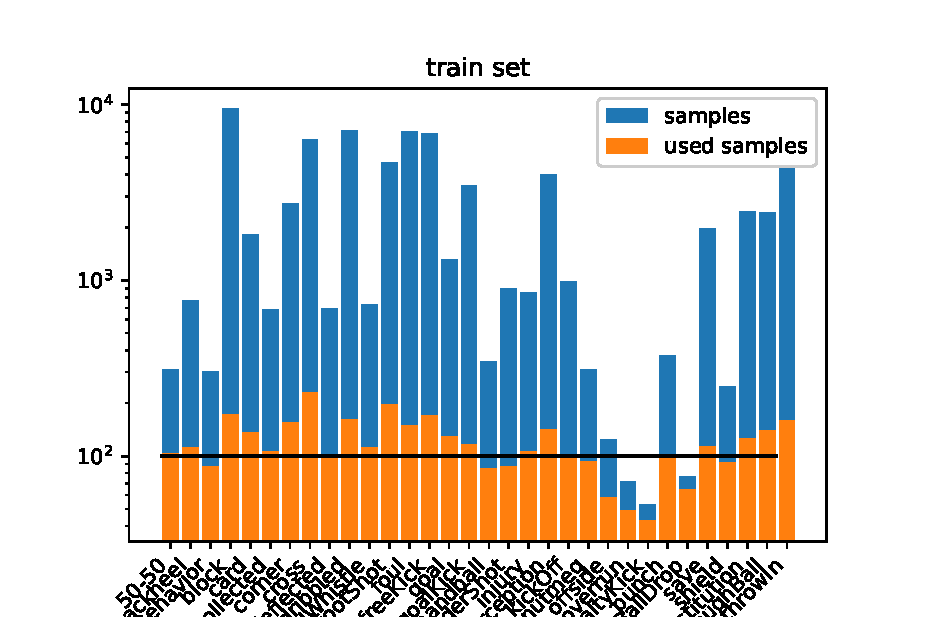
\includegraphics[width=.6\linewidth]{img/data-plots/4sec/class_distribution_used_samples_train_202010-1419-3803.eps}
    \caption{Beispielhaftes Resampling des Trainings-Sets (bei $\gls{tld:Delta} = 4.0$)}
    \label{fig:resamples}
\end{figure}

\subsection{Data Augmentation \& Standardisierung}
\label{subsec:data-augmentation}

Zu jeder Epoche werden je nach Batch-Größe mehrere Samples aus $D_{\text{train}}$, $D_\text{val}$ \bzw $D_\text{test}$ bestimmt.
Für jedes der Samples werden die jeweiligen Frames aus den Quellvideos dekodiert.

Data Augmentation beschreibt die Technik zusätzliche Trainingsdaten zu erlangen, indem zufällige Variationen gleicher Samples generiert werden (\cite{Gugger20}).
Durch den Einsatz der Temporal Augmentation wurden bereits zusätzliche Samples generiert, um Ungleichgewichtungen vorzubeugen, weshalb es keiner zusätzlichen Daten bedarf.
Jedoch können die Samples mit Methoden der gewöhnlichen Data Augmentation kombiniert werden um ein Overfitting auf teilweise (im Sinne von Überschneidungen) gleichen Samples zu verhindern.

Im Zuge der Data Augmentation wird jeder \gls{clip}, nachdem er dekodiert wurde, zunächst auf 90 \% seiner Höhe und Breite zufällig zugeschnitten.
Anschließend werden Helligkeit, Kontrast und Sättigung leicht verändert (Jittering; siehe~\cite{Tran18}).
In der Hälfte der Fälle wird das Bild horizontal gespiegelt.
Abschließend wird das Bild auf die Zielauflösung des jeweils verwendeten \gls{har}-Backbones verkleinert.
Für das Validierungs- und Testset wird nur ein 90 \%-iger zentraler Ausschnitt des Bildes erfasst und auf die Zielauflösung geschrumpft.
\autoref{fig:sample_example} zeigt ein beispielhaftes Sample nach Durchlaufen der Pre-Processing-Pipeline (bis einschließlich Data-Augmentation).

\begin{figure}
    \centering
    \includegraphics[width=.8\linewidth]{img/05_sample_example.png}
    \caption{Beispielhaftes Samples eines Eckstoßes bestehend aus 32 Frames}
    \label{fig:sample_example}
\end{figure}

Nach der Data Augmentation werden alle Tensoren standardisiert.
\Dh alle Samples werden auf einen Wertebereich von $\left[ -1, 1\right]$ projiziert -- mit einer Normalverteilung mit Mittelwert $\mu = 0$ und Standardabweichung $\sigma = 1$~\cite{Burkov19}.
Die Standardisierung erfolgt mit den Mittelwerten und Standardabweichung der vortrainierten Daten (\zB Kinetics) oder sofern nicht verfügbar mit den selbst ermittelten Werten des Datensets.
Anschließend werden die Werte auf den Bereich $\left[0, 1\right]$ normalisiert.
